\documentclass[1p]{elsarticle_modified}
%\bibliographystyle{elsarticle-num}

%\usepackage[colorlinks]{hyperref}
%\usepackage{abbrmath_seonhwa} %\Abb, \Ascr, \Acal ,\Abf, \Afrak
\usepackage{amsfonts}
\usepackage{amssymb}
\usepackage{amsmath}
\usepackage{amsthm}
\usepackage{scalefnt}
\usepackage{amsbsy}
\usepackage{kotex}
\usepackage{caption}
\usepackage{subfig}
\usepackage{color}
\usepackage{graphicx}
\usepackage{xcolor} %% white, black, red, green, blue, cyan, magenta, yellow
\usepackage{float}
\usepackage{setspace}
\usepackage{hyperref}

\usepackage{tikz}
\usetikzlibrary{arrows}

\usepackage{multirow}
\usepackage{array} % fixed length table
\usepackage{hhline}

%%%%%%%%%%%%%%%%%%%%%
\makeatletter
\renewcommand*\env@matrix[1][\arraystretch]{%
	\edef\arraystretch{#1}%
	\hskip -\arraycolsep
	\let\@ifnextchar\new@ifnextchar
	\array{*\c@MaxMatrixCols c}}
\makeatother %https://tex.stackexchange.com/questions/14071/how-can-i-increase-the-line-spacing-in-a-matrix
%%%%%%%%%%%%%%%

\usepackage[normalem]{ulem}

\newcommand{\msout}[1]{\ifmmode\text{\sout{\ensuremath{#1}}}\else\sout{#1}\fi}
%SOURCE: \msout is \stkout macro in https://tex.stackexchange.com/questions/20609/strikeout-in-math-mode

\newcommand{\cancel}[1]{
	\ifmmode
	{\color{red}\msout{#1}}
	\else
	{\color{red}\sout{#1}}
	\fi
}

\newcommand{\add}[1]{
	{\color{blue}\uwave{#1}}
}

\newcommand{\replace}[2]{
	\ifmmode
	{\color{red}\msout{#1}}{\color{blue}\uwave{#2}}
	\else
	{\color{red}\sout{#1}}{\color{blue}\uwave{#2}}
	\fi
}

\newcommand{\Sol}{\mathcal{S}} %segment
\newcommand{\D}{D} %diagram
\newcommand{\A}{\mathcal{A}} %arc


%%%%%%%%%%%%%%%%%%%%%%%%%%%%%5 test

\def\sl{\operatorname{\textup{SL}}(2,\Cbb)}
\def\psl{\operatorname{\textup{PSL}}(2,\Cbb)}
\def\quan{\mkern 1mu \triangleright \mkern 1mu}

\theoremstyle{definition}
\newtheorem{thm}{Theorem}[section]
\newtheorem{prop}[thm]{Proposition}
\newtheorem{lem}[thm]{Lemma}
\newtheorem{ques}[thm]{Question}
\newtheorem{cor}[thm]{Corollary}
\newtheorem{defn}[thm]{Definition}
\newtheorem{exam}[thm]{Example}
\newtheorem{rmk}[thm]{Remark}
\newtheorem{alg}[thm]{Algorithm}

\newcommand{\I}{\sqrt{-1}}
\begin{document}

%\begin{frontmatter}
%
%\title{Boundary parabolic representations of knots up to 8 crossings}
%
%%% Group authors per affiliation:
%\author{Yunhi Cho} 
%\address{Department of Mathematics, University of Seoul, Seoul, Korea}
%\ead{yhcho@uos.ac.kr}
%
%
%\author{Seonhwa Kim} %\fnref{s_kim}}
%\address{Center for Geometry and Physics, Institute for Basic Science, Pohang, 37673, Korea}
%\ead{ryeona17@ibs.re.kr}
%
%\author{Hyuk Kim}
%\address{Department of Mathematical Sciences, Seoul National University, Seoul 08826, Korea}
%\ead{hyukkim@snu.ac.kr}
%
%\author{Seokbeom Yoon}
%\address{Department of Mathematical Sciences, Seoul National University, Seoul, 08826,  Korea}
%\ead{sbyoon15@snu.ac.kr}
%
%\begin{abstract}
%We find all boundary parabolic representation of knots up to 8 crossings.
%
%\end{abstract}
%\begin{keyword}
%    \MSC[2010] 57M25 
%\end{keyword}
%
%\end{frontmatter}

%\linenumbers
%\tableofcontents
%
\newcommand\colored[1]{\textcolor{white}{\rule[-0.35ex]{0.8em}{1.4ex}}\kern-0.8em\color{red} #1}%
%\newcommand\colored[1]{\textcolor{white}{ #1}\kern-2.17ex	\textcolor{white}{ #1}\kern-1.81ex	\textcolor{white}{ #1}\kern-2.15ex\color{red}#1	}

{\Large $\underline{12a_{0336}~(K12a_{0336})}$}

\setlength{\tabcolsep}{10pt}
\renewcommand{\arraystretch}{1.6}
\vspace{1cm}\begin{tabular}{m{100pt}>{\centering\arraybackslash}m{274pt}}
\multirow{5}{120pt}{
	\centering
	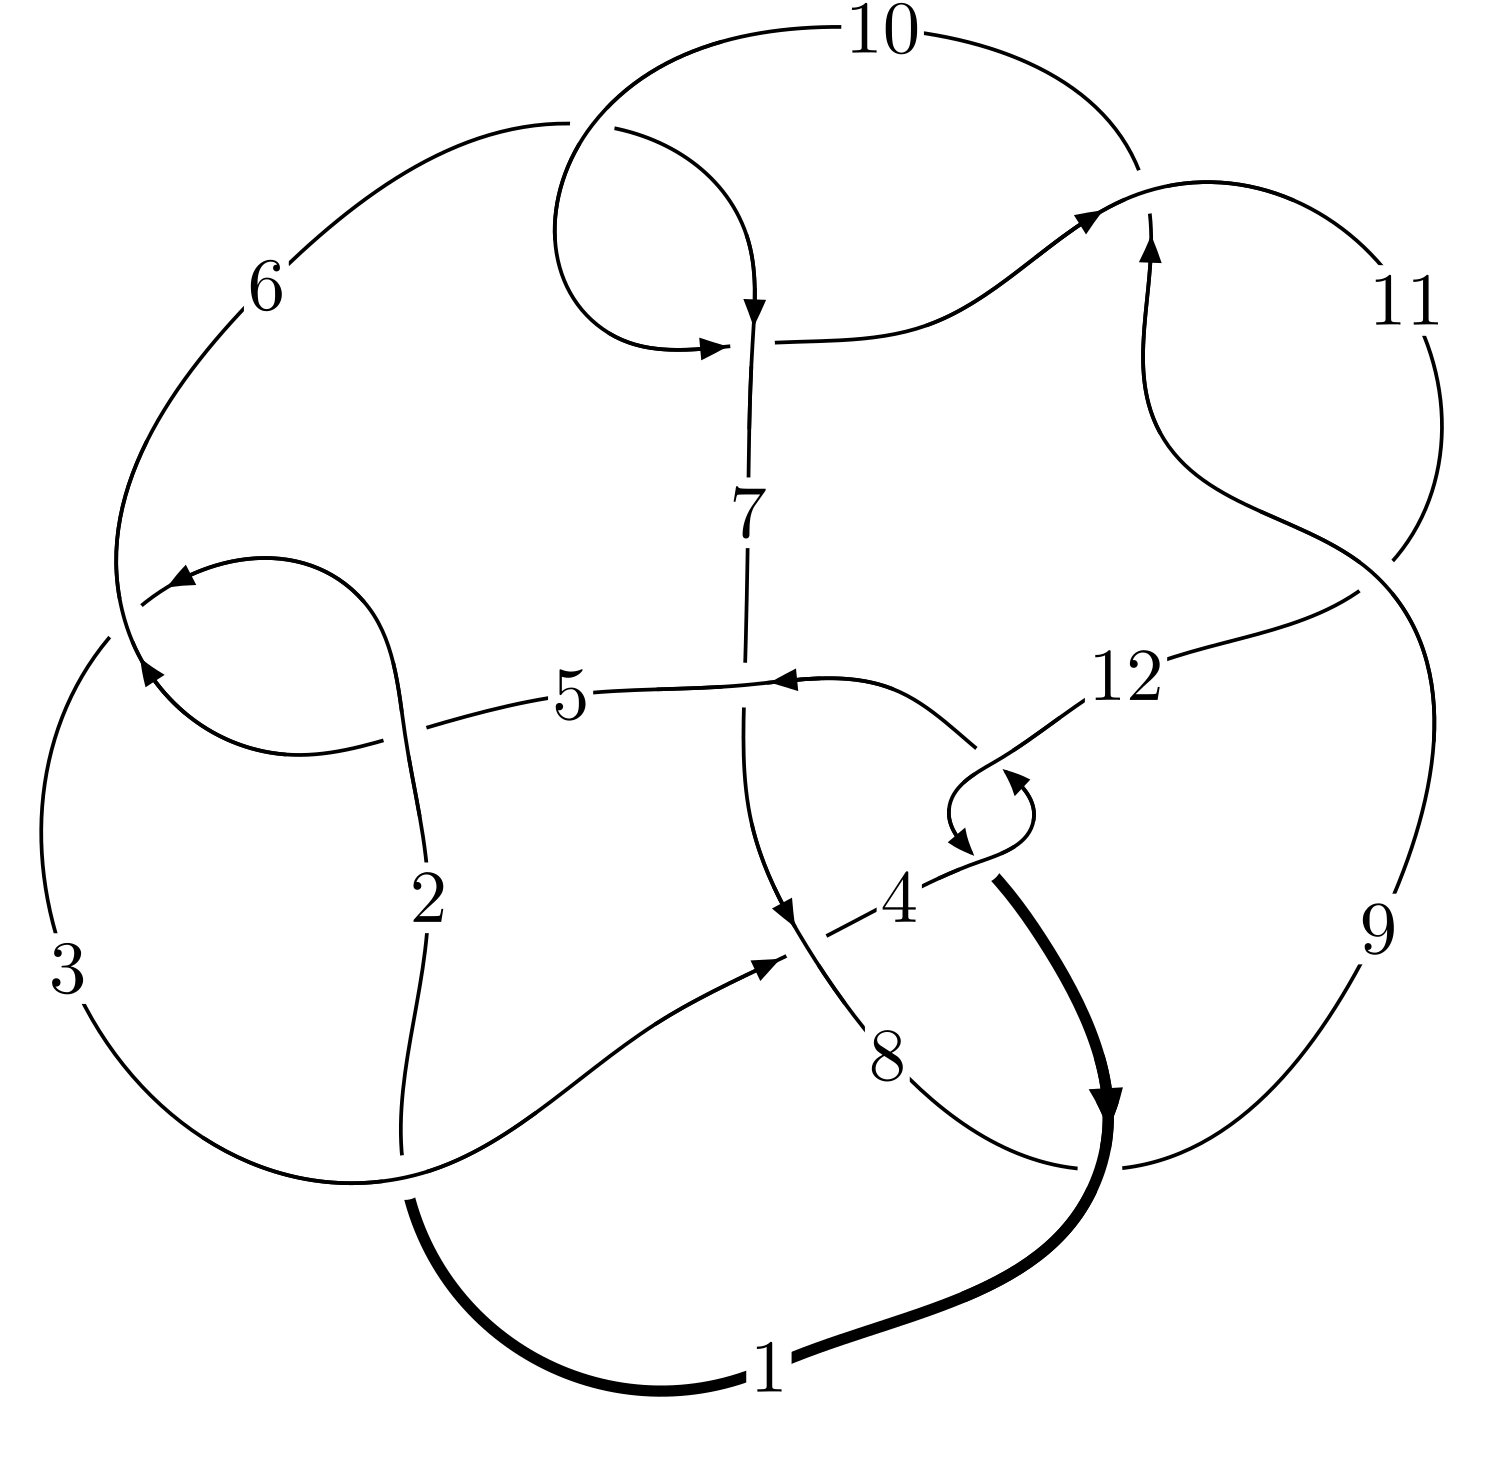
\includegraphics[width=112pt]{../../../GIT/diagram.site/Diagrams/png/1137_12a_0336.png}\\
\ \ \ A knot diagram\footnotemark}&
\allowdisplaybreaks
\textbf{Linearized knot diagam} \\
\cline{2-2}
 &
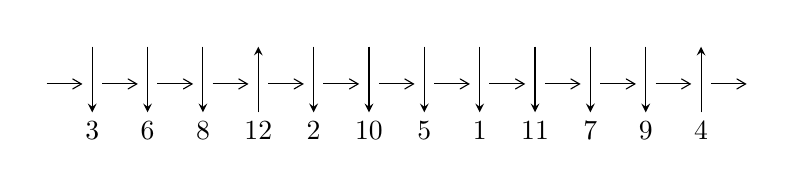
\begin{tikzpicture}[x=20pt, y=17pt]
	% nodes
	\node (C0) at (0, 0) {};
	\node (C1) at (1, 0) {};
	\node (C1U) at (1, +1) {};
	\node (C1D) at (1, -1) {3};

	\node (C2) at (2, 0) {};
	\node (C2U) at (2, +1) {};
	\node (C2D) at (2, -1) {6};

	\node (C3) at (3, 0) {};
	\node (C3U) at (3, +1) {};
	\node (C3D) at (3, -1) {8};

	\node (C4) at (4, 0) {};
	\node (C4U) at (4, +1) {};
	\node (C4D) at (4, -1) {12};

	\node (C5) at (5, 0) {};
	\node (C5U) at (5, +1) {};
	\node (C5D) at (5, -1) {2};

	\node (C6) at (6, 0) {};
	\node (C6U) at (6, +1) {};
	\node (C6D) at (6, -1) {10};

	\node (C7) at (7, 0) {};
	\node (C7U) at (7, +1) {};
	\node (C7D) at (7, -1) {5};

	\node (C8) at (8, 0) {};
	\node (C8U) at (8, +1) {};
	\node (C8D) at (8, -1) {1};

	\node (C9) at (9, 0) {};
	\node (C9U) at (9, +1) {};
	\node (C9D) at (9, -1) {11};

	\node (C10) at (10, 0) {};
	\node (C10U) at (10, +1) {};
	\node (C10D) at (10, -1) {7};

	\node (C11) at (11, 0) {};
	\node (C11U) at (11, +1) {};
	\node (C11D) at (11, -1) {9};

	\node (C12) at (12, 0) {};
	\node (C12U) at (12, +1) {};
	\node (C12D) at (12, -1) {4};
	\node (C13) at (13, 0) {};

	% arrows
	\draw[->,>={angle 60}]
	(C0) edge (C1) (C1) edge (C2) (C2) edge (C3) (C3) edge (C4) (C4) edge (C5) (C5) edge (C6) (C6) edge (C7) (C7) edge (C8) (C8) edge (C9) (C9) edge (C10) (C10) edge (C11) (C11) edge (C12) (C12) edge (C13) ;	\draw[->,>=stealth]
	(C1U) edge (C1D) (C2U) edge (C2D) (C3U) edge (C3D) (C4D) edge (C4U) (C5U) edge (C5D) (C6U) edge (C6D) (C7U) edge (C7D) (C8U) edge (C8D) (C9U) edge (C9D) (C10U) edge (C10D) (C11U) edge (C11D) (C12D) edge (C12U) ;
	\end{tikzpicture} \\
\hhline{~~} \\& 
\textbf{Solving Sequence} \\ \cline{2-2} 
 &
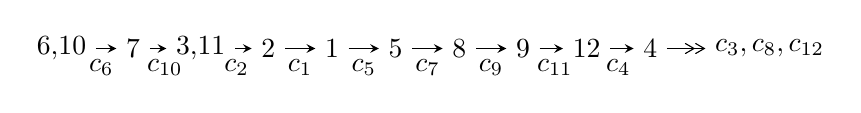
\begin{tikzpicture}[x=23pt, y=7pt]
	% node
	\node (A0) at (-1/8, 0) {6,10};
	\node (A1) at (1, 0) {7};
	\node (A2) at (33/16, 0) {3,11};
	\node (A3) at (25/8, 0) {2};
	\node (A4) at (33/8, 0) {1};
	\node (A5) at (41/8, 0) {5};
	\node (A6) at (49/8, 0) {8};
	\node (A7) at (57/8, 0) {9};
	\node (A8) at (65/8, 0) {12};
	\node (A9) at (73/8, 0) {4};
	\node (C1) at (1/2, -1) {$c_{6}$};
	\node (C2) at (3/2, -1) {$c_{10}$};
	\node (C3) at (21/8, -1) {$c_{2}$};
	\node (C4) at (29/8, -1) {$c_{1}$};
	\node (C5) at (37/8, -1) {$c_{5}$};
	\node (C6) at (45/8, -1) {$c_{7}$};
	\node (C7) at (53/8, -1) {$c_{9}$};
	\node (C8) at (61/8, -1) {$c_{11}$};
	\node (C9) at (69/8, -1) {$c_{4}$};
	\node (A10) at (11, 0) {$c_{3},c_{8},c_{12}$};

	% edge
	\draw[->,>=stealth]	
	(A0) edge (A1) (A1) edge (A2) (A2) edge (A3) (A3) edge (A4) (A4) edge (A5) (A5) edge (A6) (A6) edge (A7) (A7) edge (A8) (A8) edge (A9) ;
	\draw[->>,>={angle 60}]	
	(A9) edge (A10);
\end{tikzpicture} \\ 

\end{tabular} \\

\footnotetext{
The image of knot diagram is generated by the software ``\textbf{Draw programme}" developed by Andrew Bartholomew(\url{http://www.layer8.co.uk/maths/draw/index.htm\#Running-draw}), where we modified some parts for our purpose(\url{https://github.com/CATsTAILs/LinksPainter}).
}\phantom \\ \newline 
\centering \textbf{Ideals for irreducible components\footnotemark of $X_{\text{par}}$} 
 
\begin{align*}
I^u_{1}&=\langle 
-7.41051\times10^{147} u^{109}+3.15130\times10^{148} u^{108}+\cdots+1.10390\times10^{146} b-1.00649\times10^{148},\\
\phantom{I^u_{1}}&\phantom{= \langle  }-2.27130\times10^{149} u^{109}+9.67001\times10^{149} u^{108}+\cdots+1.10390\times10^{146} a-3.03972\times10^{149},\\
\phantom{I^u_{1}}&\phantom{= \langle  }u^{110}-5 u^{109}+\cdots+21 u-1\rangle \\
I^u_{2}&=\langle 
a^3-4 a^2+15 b-5 a+9,\;a^4-2 a^3-3 a^2+4 a+13,\;u-1\rangle \\
\\
\end{align*}
\raggedright * 2 irreducible components of $\dim_{\mathbb{C}}=0$, with total 114 representations.\\
\footnotetext{All coefficients of polynomials are rational numbers. But the coefficients are sometimes approximated in decimal forms when there is not enough margin.}
\newpage
\renewcommand{\arraystretch}{1}
\centering \section*{I. $I^u_{1}= \langle -7.41\times10^{147} u^{109}+3.15\times10^{148} u^{108}+\cdots+1.10\times10^{146} b-1.01\times10^{148},\;-2.27\times10^{149} u^{109}+9.67\times10^{149} u^{108}+\cdots+1.10\times10^{146} a-3.04\times10^{149},\;u^{110}-5 u^{109}+\cdots+21 u-1 \rangle$}
\flushleft \textbf{(i) Arc colorings}\\
\begin{tabular}{m{7pt} m{180pt} m{7pt} m{180pt} }
\flushright $a_{6}=$&$\begin{pmatrix}1\\0\end{pmatrix}$ \\
\flushright $a_{10}=$&$\begin{pmatrix}0\\u\end{pmatrix}$ \\
\flushright $a_{7}=$&$\begin{pmatrix}1\\u^2\end{pmatrix}$ \\
\flushright $a_{3}=$&$\begin{pmatrix}2057.53 u^{109}-8759.90 u^{108}+\cdots-54177.9 u+2753.63\\67.1306 u^{109}-285.471 u^{108}+\cdots-1791.59 u+91.1766\end{pmatrix}$ \\
\flushright $a_{11}=$&$\begin{pmatrix}- u\\- u^3+u\end{pmatrix}$ \\
\flushright $a_{2}=$&$\begin{pmatrix}2124.67 u^{109}-9045.37 u^{108}+\cdots-55969.5 u+2844.81\\67.1306 u^{109}-285.471 u^{108}+\cdots-1791.59 u+91.1766\end{pmatrix}$ \\
\flushright $a_{1}=$&$\begin{pmatrix}2965.90 u^{109}-12627.4 u^{108}+\cdots-78707.9 u+4024.00\\-70.4088 u^{109}+299.167 u^{108}+\cdots+1873.07 u-97.4129\end{pmatrix}$ \\
\flushright $a_{5}=$&$\begin{pmatrix}-810.769 u^{109}+3459.40 u^{108}+\cdots+22092.2 u-1136.72\\-115.246 u^{109}+490.899 u^{108}+\cdots+3011.85 u-152.033\end{pmatrix}$ \\
\flushright $a_{8}=$&$\begin{pmatrix}15726.1 u^{109}-66994.2 u^{108}+\cdots-418011. u+21301.1\\1274.16 u^{109}-5422.15 u^{108}+\cdots-33586.8 u+1705.78\end{pmatrix}$ \\
\flushright $a_{9}=$&$\begin{pmatrix}u^3\\u^5- u^3+u\end{pmatrix}$ \\
\flushright $a_{12}=$&$\begin{pmatrix}- u^5- u\\- u^7+u^5-2 u^3+u\end{pmatrix}$ \\
\flushright $a_{4}=$&$\begin{pmatrix}-675.156 u^{109}+2881.24 u^{108}+\cdots+18481.2 u-952.732\\-118.945 u^{109}+506.489 u^{108}+\cdots+3109.35 u-157.208\end{pmatrix}$\\&\end{tabular}
\flushleft \textbf{(ii) Obstruction class $= -1$}\\~\\
\flushleft \textbf{(iii) Cusp Shapes $= -1639.99 u^{109}+6951.33 u^{108}+\cdots+42540.4 u-2173.88$}\\~\\
\newpage\renewcommand{\arraystretch}{1}
\flushleft \textbf{(iv) u-Polynomials at the component}\newline \\
\begin{tabular}{m{50pt}|m{274pt}}
Crossings & \hspace{64pt}u-Polynomials at each crossing \\
\hline $$\begin{aligned}c_{1}\end{aligned}$$&$\begin{aligned}
&u^{110}+41 u^{109}+\cdots+233 u+4
\end{aligned}$\\
\hline $$\begin{aligned}c_{2},c_{5}\end{aligned}$$&$\begin{aligned}
&u^{110}+7 u^{109}+\cdots+27 u+2
\end{aligned}$\\
\hline $$\begin{aligned}c_{3}\end{aligned}$$&$\begin{aligned}
&u^{110}+u^{109}+\cdots+17 u-1
\end{aligned}$\\
\hline $$\begin{aligned}c_{4},c_{12}\end{aligned}$$&$\begin{aligned}
&u^{110}+7 u^{109}+\cdots+27 u+1
\end{aligned}$\\
\hline $$\begin{aligned}c_{6},c_{10}\end{aligned}$$&$\begin{aligned}
&u^{110}+5 u^{109}+\cdots-21 u-1
\end{aligned}$\\
\hline $$\begin{aligned}c_{7}\end{aligned}$$&$\begin{aligned}
&u^{110}+25 u^{109}+\cdots+376147 u-1476493
\end{aligned}$\\
\hline $$\begin{aligned}c_{8}\end{aligned}$$&$\begin{aligned}
&u^{110}+5 u^{109}+\cdots-101 u+41
\end{aligned}$\\
\hline $$\begin{aligned}c_{9},c_{11}\end{aligned}$$&$\begin{aligned}
&u^{110}+35 u^{109}+\cdots+127 u+1
\end{aligned}$\\
\hline
\end{tabular}\\~\\
\newpage\renewcommand{\arraystretch}{1}
\flushleft \textbf{(v) Riley Polynomials at the component}\newline \\
\begin{tabular}{m{50pt}|m{274pt}}
Crossings & \hspace{64pt}Riley Polynomials at each crossing \\
\hline $$\begin{aligned}c_{1}\end{aligned}$$&$\begin{aligned}
&y^{110}+59 y^{109}+\cdots-9873 y+16
\end{aligned}$\\
\hline $$\begin{aligned}c_{2},c_{5}\end{aligned}$$&$\begin{aligned}
&y^{110}-41 y^{109}+\cdots-233 y+4
\end{aligned}$\\
\hline $$\begin{aligned}c_{3}\end{aligned}$$&$\begin{aligned}
&y^{110}-3 y^{109}+\cdots-79 y+1
\end{aligned}$\\
\hline $$\begin{aligned}c_{4},c_{12}\end{aligned}$$&$\begin{aligned}
&y^{110}+65 y^{109}+\cdots-175 y+1
\end{aligned}$\\
\hline $$\begin{aligned}c_{6},c_{10}\end{aligned}$$&$\begin{aligned}
&y^{110}-35 y^{109}+\cdots-127 y+1
\end{aligned}$\\
\hline $$\begin{aligned}c_{7}\end{aligned}$$&$\begin{aligned}
&y^{110}-145 y^{109}+\cdots+12275866812167 y+2180031579049
\end{aligned}$\\
\hline $$\begin{aligned}c_{8}\end{aligned}$$&$\begin{aligned}
&y^{110}+155 y^{109}+\cdots+197587 y+1681
\end{aligned}$\\
\hline $$\begin{aligned}c_{9},c_{11}\end{aligned}$$&$\begin{aligned}
&y^{110}+85 y^{109}+\cdots-2511 y+1
\end{aligned}$\\
\hline
\end{tabular}\\~\\
\newpage\flushleft \textbf{(vi) Complex Volumes and Cusp Shapes}
$$\begin{array}{c|c|c}  
\text{Solutions to }I^u_{1}& \I (\text{vol} + \sqrt{-1}CS) & \text{Cusp shape}\\
 \hline 
\begin{aligned}
u &= \phantom{-}0.990959 + 0.098136 I \\
a &= \phantom{-}1.275900 - 0.543178 I \\
b &= \phantom{-}0.892858 - 0.506092 I\end{aligned}
 & -1.69575 + 2.02020 I & \phantom{-0.000000 } 0 \\ \hline\begin{aligned}
u &= \phantom{-}0.990959 - 0.098136 I \\
a &= \phantom{-}1.275900 + 0.543178 I \\
b &= \phantom{-}0.892858 + 0.506092 I\end{aligned}
 & -1.69575 - 2.02020 I & \phantom{-0.000000 } 0 \\ \hline\begin{aligned}
u &= \phantom{-}0.996189 + 0.199368 I \\
a &= -0.337539 + 1.135930 I \\
b &= -0.212986 - 0.116839 I\end{aligned}
 & -3.59787 - 0.10583 I & \phantom{-0.000000 } 0 \\ \hline\begin{aligned}
u &= \phantom{-}0.996189 - 0.199368 I \\
a &= -0.337539 - 1.135930 I \\
b &= -0.212986 + 0.116839 I\end{aligned}
 & -3.59787 + 0.10583 I & \phantom{-0.000000 } 0 \\ \hline\begin{aligned}
u &= -0.774665 + 0.664449 I \\
a &= -1.25947 - 0.88402 I \\
b &= -0.926563 - 0.223291 I\end{aligned}
 & -0.205553 - 0.307982 I & \phantom{-0.000000 } 0 \\ \hline\begin{aligned}
u &= -0.774665 - 0.664449 I \\
a &= -1.25947 + 0.88402 I \\
b &= -0.926563 + 0.223291 I\end{aligned}
 & -0.205553 + 0.307982 I & \phantom{-0.000000 } 0 \\ \hline\begin{aligned}
u &= -0.993094 + 0.295258 I \\
a &= \phantom{-}1.55343 + 1.20146 I \\
b &= \phantom{-}1.079160 - 0.620858 I\end{aligned}
 & -0.75551 + 7.78682 I & \phantom{-0.000000 } 0 \\ \hline\begin{aligned}
u &= -0.993094 - 0.295258 I \\
a &= \phantom{-}1.55343 - 1.20146 I \\
b &= \phantom{-}1.079160 + 0.620858 I\end{aligned}
 & -0.75551 - 7.78682 I & \phantom{-0.000000 } 0 \\ \hline\begin{aligned}
u &= \phantom{-}0.697332 + 0.792742 I \\
a &= -0.246586 - 0.264787 I \\
b &= \phantom{-}1.220130 - 0.142302 I\end{aligned}
 & -2.44609 + 5.13634 I & \phantom{-0.000000 } 0 \\ \hline\begin{aligned}
u &= \phantom{-}0.697332 - 0.792742 I \\
a &= -0.246586 + 0.264787 I \\
b &= \phantom{-}1.220130 + 0.142302 I\end{aligned}
 & -2.44609 - 5.13634 I & \phantom{-0.000000 } 0\\
 \hline 
 \end{array}$$\newpage$$\begin{array}{c|c|c}  
\text{Solutions to }I^u_{1}& \I (\text{vol} + \sqrt{-1}CS) & \text{Cusp shape}\\
 \hline 
\begin{aligned}
u &= -1.062770 + 0.148015 I \\
a &= \phantom{-}1.58044 + 0.11499 I \\
b &= \phantom{-}1.175380 + 0.017061 I\end{aligned}
 & -8.83330 + 5.21023 I & \phantom{-0.000000 } 0 \\ \hline\begin{aligned}
u &= -1.062770 - 0.148015 I \\
a &= \phantom{-}1.58044 - 0.11499 I \\
b &= \phantom{-}1.175380 - 0.017061 I\end{aligned}
 & -8.83330 - 5.21023 I & \phantom{-0.000000 } 0 \\ \hline\begin{aligned}
u &= -0.843116 + 0.333311 I \\
a &= -0.284924 + 0.220862 I \\
b &= \phantom{-}0.392082 + 0.747113 I\end{aligned}
 & \phantom{-}1.15133 + 2.61903 I & \phantom{-0.000000 } 0 \\ \hline\begin{aligned}
u &= -0.843116 - 0.333311 I \\
a &= -0.284924 - 0.220862 I \\
b &= \phantom{-}0.392082 - 0.747113 I\end{aligned}
 & \phantom{-}1.15133 - 2.61903 I & \phantom{-0.000000 } 0 \\ \hline\begin{aligned}
u &= -0.622477 + 0.901671 I \\
a &= -0.341590 - 1.224490 I \\
b &= \phantom{-}0.916045 + 0.686391 I\end{aligned}
 & \phantom{-}4.73684 - 3.99325 I & \phantom{-0.000000 } 0 \\ \hline\begin{aligned}
u &= -0.622477 - 0.901671 I \\
a &= -0.341590 + 1.224490 I \\
b &= \phantom{-}0.916045 - 0.686391 I\end{aligned}
 & \phantom{-}4.73684 + 3.99325 I & \phantom{-0.000000 } 0 \\ \hline\begin{aligned}
u &= -0.902097\phantom{ +0.000000I} \\
a &= -1.76787\phantom{ +0.000000I} \\
b &= -1.24916\phantom{ +0.000000I}\end{aligned}
 & -4.50976\phantom{ +0.000000I} & \phantom{-0.000000 } 0 \\ \hline\begin{aligned}
u &= \phantom{-}0.835064 + 0.721373 I \\
a &= \phantom{-}1.47161 - 1.06013 I \\
b &= -1.002620 + 0.908716 I\end{aligned}
 & \phantom{-}0.330530 + 0.796888 I & \phantom{-0.000000 } 0 \\ \hline\begin{aligned}
u &= \phantom{-}0.835064 - 0.721373 I \\
a &= \phantom{-}1.47161 + 1.06013 I \\
b &= -1.002620 - 0.908716 I\end{aligned}
 & \phantom{-}0.330530 - 0.796888 I & \phantom{-0.000000 } 0 \\ \hline\begin{aligned}
u &= \phantom{-}0.867770 + 0.692580 I \\
a &= \phantom{-}0.634138 + 0.236501 I \\
b &= -1.313380 + 0.439862 I\end{aligned}
 & -0.77993 - 1.27179 I & \phantom{-0.000000 } 0\\
 \hline 
 \end{array}$$\newpage$$\begin{array}{c|c|c}  
\text{Solutions to }I^u_{1}& \I (\text{vol} + \sqrt{-1}CS) & \text{Cusp shape}\\
 \hline 
\begin{aligned}
u &= \phantom{-}0.867770 - 0.692580 I \\
a &= \phantom{-}0.634138 - 0.236501 I \\
b &= -1.313380 - 0.439862 I\end{aligned}
 & -0.77993 + 1.27179 I & \phantom{-0.000000 } 0 \\ \hline\begin{aligned}
u &= -0.878182 + 0.681537 I \\
a &= \phantom{-}0.533325 + 0.497799 I \\
b &= \phantom{-}0.686950 + 0.106206 I\end{aligned}
 & \phantom{-}2.03663 + 2.63082 I & \phantom{-0.000000 } 0 \\ \hline\begin{aligned}
u &= -0.878182 - 0.681537 I \\
a &= \phantom{-}0.533325 - 0.497799 I \\
b &= \phantom{-}0.686950 - 0.106206 I\end{aligned}
 & \phantom{-}2.03663 - 2.63082 I & \phantom{-0.000000 } 0 \\ \hline\begin{aligned}
u &= \phantom{-}0.813749 + 0.768223 I \\
a &= \phantom{-}0.99853 - 1.18681 I \\
b &= -0.290691 + 1.035300 I\end{aligned}
 & \phantom{-}3.09414 + 1.62165 I & \phantom{-0.000000 } 0 \\ \hline\begin{aligned}
u &= \phantom{-}0.813749 - 0.768223 I \\
a &= \phantom{-}0.99853 + 1.18681 I \\
b &= -0.290691 - 1.035300 I\end{aligned}
 & \phantom{-}3.09414 - 1.62165 I & \phantom{-0.000000 } 0 \\ \hline\begin{aligned}
u &= \phantom{-}0.081059 + 0.876379 I \\
a &= \phantom{-}0.42575 + 1.39611 I \\
b &= -1.013040 - 0.658910 I\end{aligned}
 & -0.50846 - 8.74088 I & \phantom{-0.000000 } 0 \\ \hline\begin{aligned}
u &= \phantom{-}0.081059 - 0.876379 I \\
a &= \phantom{-}0.42575 - 1.39611 I \\
b &= -1.013040 + 0.658910 I\end{aligned}
 & -0.50846 + 8.74088 I & \phantom{-0.000000 } 0 \\ \hline\begin{aligned}
u &= \phantom{-}0.885644 + 0.691977 I \\
a &= -0.05764 + 1.73251 I \\
b &= -1.333450 - 0.331323 I\end{aligned}
 & -0.83704 - 4.05265 I & \phantom{-0.000000 } 0 \\ \hline\begin{aligned}
u &= \phantom{-}0.885644 - 0.691977 I \\
a &= -0.05764 - 1.73251 I \\
b &= -1.333450 + 0.331323 I\end{aligned}
 & -0.83704 + 4.05265 I & \phantom{-0.000000 } 0 \\ \hline\begin{aligned}
u &= -1.092140 + 0.284265 I \\
a &= \phantom{-}0.240713 - 0.003212 I \\
b &= -0.495383 - 0.799993 I\end{aligned}
 & -3.02604 + 7.06344 I & \phantom{-0.000000 } 0\\
 \hline 
 \end{array}$$\newpage$$\begin{array}{c|c|c}  
\text{Solutions to }I^u_{1}& \I (\text{vol} + \sqrt{-1}CS) & \text{Cusp shape}\\
 \hline 
\begin{aligned}
u &= -1.092140 - 0.284265 I \\
a &= \phantom{-}0.240713 + 0.003212 I \\
b &= -0.495383 + 0.799993 I\end{aligned}
 & -3.02604 - 7.06344 I & \phantom{-0.000000 } 0 \\ \hline\begin{aligned}
u &= -0.867655 + 0.040937 I \\
a &= -1.51760 - 0.61667 I \\
b &= -1.151050 + 0.669665 I\end{aligned}
 & -4.17559 + 2.45296 I & \phantom{-0.000000 } 0 \\ \hline\begin{aligned}
u &= -0.867655 - 0.040937 I \\
a &= -1.51760 + 0.61667 I \\
b &= -1.151050 - 0.669665 I\end{aligned}
 & -4.17559 - 2.45296 I & \phantom{-0.000000 } 0 \\ \hline\begin{aligned}
u &= -0.828091 + 0.780039 I \\
a &= -0.185197 + 0.072379 I \\
b &= \phantom{-}0.117195 + 0.402603 I\end{aligned}
 & \phantom{-}2.64336 + 1.65504 I & \phantom{-0.000000 } 0 \\ \hline\begin{aligned}
u &= -0.828091 - 0.780039 I \\
a &= -0.185197 - 0.072379 I \\
b &= \phantom{-}0.117195 - 0.402603 I\end{aligned}
 & \phantom{-}2.64336 - 1.65504 I & \phantom{-0.000000 } 0 \\ \hline\begin{aligned}
u &= -0.697509 + 0.900889 I \\
a &= -0.369911 + 1.319140 I \\
b &= \phantom{-}0.772510 - 0.700845 I\end{aligned}
 & \phantom{-}5.16781 + 1.33455 I & \phantom{-0.000000 } 0 \\ \hline\begin{aligned}
u &= -0.697509 - 0.900889 I \\
a &= -0.369911 - 1.319140 I \\
b &= \phantom{-}0.772510 + 0.700845 I\end{aligned}
 & \phantom{-}5.16781 - 1.33455 I & \phantom{-0.000000 } 0 \\ \hline\begin{aligned}
u &= -0.872826 + 0.738046 I \\
a &= \phantom{-}1.13776 - 5.90790 I \\
b &= \phantom{-}0.894681 + 0.537347 I\end{aligned}
 & \phantom{-}1.29270 + 0.75901 I & \phantom{-0.000000 } 0 \\ \hline\begin{aligned}
u &= -0.872826 - 0.738046 I \\
a &= \phantom{-}1.13776 + 5.90790 I \\
b &= \phantom{-}0.894681 - 0.537347 I\end{aligned}
 & \phantom{-}1.29270 - 0.75901 I & \phantom{-0.000000 } 0 \\ \hline\begin{aligned}
u &= -0.877187 + 0.735804 I \\
a &= \phantom{-}4.12267 + 5.29001 I \\
b &= \phantom{-}0.910898 - 0.520689 I\end{aligned}
 & \phantom{-}1.27829 + 4.84714 I & \phantom{-0.000000 } 0\\
 \hline 
 \end{array}$$\newpage$$\begin{array}{c|c|c}  
\text{Solutions to }I^u_{1}& \I (\text{vol} + \sqrt{-1}CS) & \text{Cusp shape}\\
 \hline 
\begin{aligned}
u &= -0.877187 - 0.735804 I \\
a &= \phantom{-}4.12267 - 5.29001 I \\
b &= \phantom{-}0.910898 + 0.520689 I\end{aligned}
 & \phantom{-}1.27829 - 4.84714 I & \phantom{-0.000000 } 0 \\ \hline\begin{aligned}
u &= \phantom{-}0.770569 + 0.856471 I \\
a &= -0.75952 + 1.22815 I \\
b &= \phantom{-}1.094710 - 0.747854 I\end{aligned}
 & \phantom{-}6.67136 + 6.50363 I & \phantom{-0.000000 } 0 \\ \hline\begin{aligned}
u &= \phantom{-}0.770569 - 0.856471 I \\
a &= -0.75952 - 1.22815 I \\
b &= \phantom{-}1.094710 + 0.747854 I\end{aligned}
 & \phantom{-}6.67136 - 6.50363 I & \phantom{-0.000000 } 0 \\ \hline\begin{aligned}
u &= \phantom{-}0.736971 + 0.887786 I \\
a &= \phantom{-}0.40009 + 1.53796 I \\
b &= -0.588057 - 0.913960 I\end{aligned}
 & \phantom{-}4.79934 + 6.61268 I & \phantom{-0.000000 } 0 \\ \hline\begin{aligned}
u &= \phantom{-}0.736971 - 0.887786 I \\
a &= \phantom{-}0.40009 - 1.53796 I \\
b &= -0.588057 + 0.913960 I\end{aligned}
 & \phantom{-}4.79934 - 6.61268 I & \phantom{-0.000000 } 0 \\ \hline\begin{aligned}
u &= \phantom{-}0.712081 + 0.909440 I \\
a &= \phantom{-}0.55860 - 1.38226 I \\
b &= -1.089970 + 0.717795 I\end{aligned}
 & \phantom{-}3.25044 + 12.62120 I & \phantom{-0.000000 } 0 \\ \hline\begin{aligned}
u &= \phantom{-}0.712081 - 0.909440 I \\
a &= \phantom{-}0.55860 + 1.38226 I \\
b &= -1.089970 - 0.717795 I\end{aligned}
 & \phantom{-}3.25044 - 12.62120 I & \phantom{-0.000000 } 0 \\ \hline\begin{aligned}
u &= -0.831776 + 0.144488 I \\
a &= -0.239608 - 0.113887 I \\
b &= -0.614202 + 0.872721 I\end{aligned}
 & -2.44902 + 3.63797 I & \phantom{-0.000000 } 0 \\ \hline\begin{aligned}
u &= -0.831776 - 0.144488 I \\
a &= -0.239608 + 0.113887 I \\
b &= -0.614202 - 0.872721 I\end{aligned}
 & -2.44902 - 3.63797 I & \phantom{-0.000000 } 0 \\ \hline\begin{aligned}
u &= \phantom{-}1.051500 + 0.482675 I \\
a &= \phantom{-}0.79964 - 1.65316 I \\
b &= \phantom{-}1.009650 + 0.153910 I\end{aligned}
 & -6.86902 - 1.41545 I & \phantom{-0.000000 } 0\\
 \hline 
 \end{array}$$\newpage$$\begin{array}{c|c|c}  
\text{Solutions to }I^u_{1}& \I (\text{vol} + \sqrt{-1}CS) & \text{Cusp shape}\\
 \hline 
\begin{aligned}
u &= \phantom{-}1.051500 - 0.482675 I \\
a &= \phantom{-}0.79964 + 1.65316 I \\
b &= \phantom{-}1.009650 - 0.153910 I\end{aligned}
 & -6.86902 + 1.41545 I & \phantom{-0.000000 } 0 \\ \hline\begin{aligned}
u &= \phantom{-}0.908591 + 0.716880 I \\
a &= -0.12317 + 2.53742 I \\
b &= -1.074790 - 0.887097 I\end{aligned}
 & \phantom{-}0.10246 - 6.29605 I & \phantom{-0.000000 } 0 \\ \hline\begin{aligned}
u &= \phantom{-}0.908591 - 0.716880 I \\
a &= -0.12317 - 2.53742 I \\
b &= -1.074790 + 0.887097 I\end{aligned}
 & \phantom{-}0.10246 + 6.29605 I & \phantom{-0.000000 } 0 \\ \hline\begin{aligned}
u &= \phantom{-}0.809732 + 0.833377 I \\
a &= -0.19331 - 1.71805 I \\
b &= \phantom{-}0.614409 + 0.971864 I\end{aligned}
 & \phantom{-}8.17677 + 0.24318 I & \phantom{-0.000000 } 0 \\ \hline\begin{aligned}
u &= \phantom{-}0.809732 - 0.833377 I \\
a &= -0.19331 + 1.71805 I \\
b &= \phantom{-}0.614409 - 0.971864 I\end{aligned}
 & \phantom{-}8.17677 - 0.24318 I & \phantom{-0.000000 } 0 \\ \hline\begin{aligned}
u &= -0.960649 + 0.654756 I \\
a &= -1.130610 - 0.112359 I \\
b &= -0.894555 + 0.088679 I\end{aligned}
 & -0.80311 + 5.44115 I & \phantom{-0.000000 } 0 \\ \hline\begin{aligned}
u &= -0.960649 - 0.654756 I \\
a &= -1.130610 + 0.112359 I \\
b &= -0.894555 - 0.088679 I\end{aligned}
 & -0.80311 - 5.44115 I & \phantom{-0.000000 } 0 \\ \hline\begin{aligned}
u &= \phantom{-}0.778635 + 0.277338 I \\
a &= -1.33414 + 2.80799 I \\
b &= -0.942986 - 0.438315 I\end{aligned}
 & -1.96405 - 2.91621 I & \phantom{-0.000000 } 0 \\ \hline\begin{aligned}
u &= \phantom{-}0.778635 - 0.277338 I \\
a &= -1.33414 - 2.80799 I \\
b &= -0.942986 + 0.438315 I\end{aligned}
 & -1.96405 + 2.91621 I & \phantom{-0.000000 } 0 \\ \hline\begin{aligned}
u &= -1.152970 + 0.265802 I \\
a &= -1.30202 - 1.16410 I \\
b &= -1.075150 + 0.649293 I\end{aligned}
 & -4.73120 + 12.50000 I & \phantom{-0.000000 } 0\\
 \hline 
 \end{array}$$\newpage$$\begin{array}{c|c|c}  
\text{Solutions to }I^u_{1}& \I (\text{vol} + \sqrt{-1}CS) & \text{Cusp shape}\\
 \hline 
\begin{aligned}
u &= -1.152970 - 0.265802 I \\
a &= -1.30202 + 1.16410 I \\
b &= -1.075150 - 0.649293 I\end{aligned}
 & -4.73120 - 12.50000 I & \phantom{-0.000000 } 0 \\ \hline\begin{aligned}
u &= \phantom{-}0.007248 + 0.810052 I \\
a &= \phantom{-}0.37732 - 1.38238 I \\
b &= -0.618881 + 0.726901 I\end{aligned}
 & \phantom{-}0.65865 - 3.42633 I & \phantom{-0.000000 } 0 \\ \hline\begin{aligned}
u &= \phantom{-}0.007248 - 0.810052 I \\
a &= \phantom{-}0.37732 + 1.38238 I \\
b &= -0.618881 - 0.726901 I\end{aligned}
 & \phantom{-}0.65865 + 3.42633 I & \phantom{-0.000000 } 0 \\ \hline\begin{aligned}
u &= \phantom{-}0.931716 + 0.744804 I \\
a &= -0.48784 + 1.54283 I \\
b &= -0.365752 - 1.068560 I\end{aligned}
 & \phantom{-}2.73350 - 7.34740 I & \phantom{-0.000000 } 0 \\ \hline\begin{aligned}
u &= \phantom{-}0.931716 - 0.744804 I \\
a &= -0.48784 - 1.54283 I \\
b &= -0.365752 + 1.068560 I\end{aligned}
 & \phantom{-}2.73350 + 7.34740 I & \phantom{-0.000000 } 0 \\ \hline\begin{aligned}
u &= -0.800702 + 0.893151 I \\
a &= \phantom{-}0.66551 + 1.27924 I \\
b &= -0.866053 - 0.674686 I\end{aligned}
 & \phantom{-}5.61155 + 0.14050 I & \phantom{-0.000000 } 0 \\ \hline\begin{aligned}
u &= -0.800702 - 0.893151 I \\
a &= \phantom{-}0.66551 - 1.27924 I \\
b &= -0.866053 + 0.674686 I\end{aligned}
 & \phantom{-}5.61155 - 0.14050 I & \phantom{-0.000000 } 0 \\ \hline\begin{aligned}
u &= -0.927118 + 0.763957 I \\
a &= \phantom{-}0.1000390 + 0.0172765 I \\
b &= \phantom{-}0.221052 - 0.379085 I\end{aligned}
 & \phantom{-}2.34244 + 4.16755 I & \phantom{-0.000000 } 0 \\ \hline\begin{aligned}
u &= -0.927118 - 0.763957 I \\
a &= \phantom{-}0.1000390 - 0.0172765 I \\
b &= \phantom{-}0.221052 + 0.379085 I\end{aligned}
 & \phantom{-}2.34244 - 4.16755 I & \phantom{-0.000000 } 0 \\ \hline\begin{aligned}
u &= \phantom{-}1.182250 + 0.265329 I \\
a &= -0.845000 + 0.942118 I \\
b &= -0.675555 - 0.540568 I\end{aligned}
 & -3.25800 - 0.36532 I & \phantom{-0.000000 } 0\\
 \hline 
 \end{array}$$\newpage$$\begin{array}{c|c|c}  
\text{Solutions to }I^u_{1}& \I (\text{vol} + \sqrt{-1}CS) & \text{Cusp shape}\\
 \hline 
\begin{aligned}
u &= \phantom{-}1.182250 - 0.265329 I \\
a &= -0.845000 - 0.942118 I \\
b &= -0.675555 + 0.540568 I\end{aligned}
 & -3.25800 + 0.36532 I & \phantom{-0.000000 } 0 \\ \hline\begin{aligned}
u &= \phantom{-}1.001380 + 0.722993 I \\
a &= \phantom{-}0.317622 - 1.284450 I \\
b &= \phantom{-}1.267730 + 0.111185 I\end{aligned}
 & -3.35621 - 10.85530 I & \phantom{-0.000000 } 0 \\ \hline\begin{aligned}
u &= \phantom{-}1.001380 - 0.722993 I \\
a &= \phantom{-}0.317622 + 1.284450 I \\
b &= \phantom{-}1.267730 - 0.111185 I\end{aligned}
 & -3.35621 + 10.85530 I & \phantom{-0.000000 } 0 \\ \hline\begin{aligned}
u &= \phantom{-}0.958427 + 0.782280 I \\
a &= -1.31241 + 0.78086 I \\
b &= \phantom{-}0.571194 - 1.000510 I\end{aligned}
 & \phantom{-}7.71445 - 6.27796 I & \phantom{-0.000000 } 0 \\ \hline\begin{aligned}
u &= \phantom{-}0.958427 - 0.782280 I \\
a &= -1.31241 - 0.78086 I \\
b &= \phantom{-}0.571194 + 1.000510 I\end{aligned}
 & \phantom{-}7.71445 + 6.27796 I & \phantom{-0.000000 } 0 \\ \hline\begin{aligned}
u &= \phantom{-}1.238090 + 0.023214 I \\
a &= \phantom{-}0.836611 + 0.344859 I \\
b &= \phantom{-}0.847431 - 0.588895 I\end{aligned}
 & -2.03804 + 2.33452 I & \phantom{-0.000000 } 0 \\ \hline\begin{aligned}
u &= \phantom{-}1.238090 - 0.023214 I \\
a &= \phantom{-}0.836611 - 0.344859 I \\
b &= \phantom{-}0.847431 + 0.588895 I\end{aligned}
 & -2.03804 - 2.33452 I & \phantom{-0.000000 } 0 \\ \hline\begin{aligned}
u &= -0.858642 + 0.897188 I \\
a &= \phantom{-}0.34642 - 1.72422 I \\
b &= -0.834452 + 0.677799 I\end{aligned}
 & \phantom{-}5.70786 + 5.35963 I & \phantom{-0.000000 } 0 \\ \hline\begin{aligned}
u &= -0.858642 - 0.897188 I \\
a &= \phantom{-}0.34642 + 1.72422 I \\
b &= -0.834452 - 0.677799 I\end{aligned}
 & \phantom{-}5.70786 - 5.35963 I & \phantom{-0.000000 } 0 \\ \hline\begin{aligned}
u &= \phantom{-}0.743069 + 0.001373 I \\
a &= -15.7688 + 14.3067 I \\
b &= \phantom{-}0.853529 + 0.493943 I\end{aligned}
 & -2.73468 - 2.03121 I & -155.856 - 14.904 I\\
 \hline 
 \end{array}$$\newpage$$\begin{array}{c|c|c}  
\text{Solutions to }I^u_{1}& \I (\text{vol} + \sqrt{-1}CS) & \text{Cusp shape}\\
 \hline 
\begin{aligned}
u &= \phantom{-}0.743069 - 0.001373 I \\
a &= -15.7688 - 14.3067 I \\
b &= \phantom{-}0.853529 - 0.493943 I\end{aligned}
 & -2.73468 + 2.03121 I & -155.856 + 14.904 I \\ \hline\begin{aligned}
u &= \phantom{-}1.204310 + 0.367220 I \\
a &= -0.293140 - 0.037779 I \\
b &= -0.979382 + 0.596671 I\end{aligned}
 & -4.22594 + 4.29044 I & \phantom{-0.000000 } 0 \\ \hline\begin{aligned}
u &= \phantom{-}1.204310 - 0.367220 I \\
a &= -0.293140 + 0.037779 I \\
b &= -0.979382 - 0.596671 I\end{aligned}
 & -4.22594 - 4.29044 I & \phantom{-0.000000 } 0 \\ \hline\begin{aligned}
u &= \phantom{-}0.991910 + 0.777202 I \\
a &= \phantom{-}0.45402 - 2.37267 I \\
b &= \phantom{-}1.124230 + 0.740932 I\end{aligned}
 & \phantom{-}5.98378 - 12.58750 I & \phantom{-0.000000 } 0 \\ \hline\begin{aligned}
u &= \phantom{-}0.991910 - 0.777202 I \\
a &= \phantom{-}0.45402 + 2.37267 I \\
b &= \phantom{-}1.124230 - 0.740932 I\end{aligned}
 & \phantom{-}5.98378 + 12.58750 I & \phantom{-0.000000 } 0 \\ \hline\begin{aligned}
u &= -0.945626 + 0.842407 I \\
a &= \phantom{-}1.095890 + 0.776380 I \\
b &= -0.783570 - 0.663137 I\end{aligned}
 & \phantom{-}5.42222 + 1.04774 I & \phantom{-0.000000 } 0 \\ \hline\begin{aligned}
u &= -0.945626 - 0.842407 I \\
a &= \phantom{-}1.095890 - 0.776380 I \\
b &= -0.783570 + 0.663137 I\end{aligned}
 & \phantom{-}5.42222 - 1.04774 I & \phantom{-0.000000 } 0 \\ \hline\begin{aligned}
u &= -0.982963 + 0.809149 I \\
a &= -0.26329 - 2.24551 I \\
b &= -0.909073 + 0.649568 I\end{aligned}
 & \phantom{-}5.03632 + 6.14721 I & \phantom{-0.000000 } 0 \\ \hline\begin{aligned}
u &= -0.982963 - 0.809149 I \\
a &= -0.26329 + 2.24551 I \\
b &= -0.909073 - 0.649568 I\end{aligned}
 & \phantom{-}5.03632 - 6.14721 I & \phantom{-0.000000 } 0 \\ \hline\begin{aligned}
u &= \phantom{-}0.270523 + 0.671458 I \\
a &= -0.265968 + 0.602362 I \\
b &= \phantom{-}1.011230 + 0.007454 I\end{aligned}
 & -4.61086 - 2.90503 I & -12.49793 + 3.69733 I\\
 \hline 
 \end{array}$$\newpage$$\begin{array}{c|c|c}  
\text{Solutions to }I^u_{1}& \I (\text{vol} + \sqrt{-1}CS) & \text{Cusp shape}\\
 \hline 
\begin{aligned}
u &= \phantom{-}0.270523 - 0.671458 I \\
a &= -0.265968 - 0.602362 I \\
b &= \phantom{-}1.011230 - 0.007454 I\end{aligned}
 & -4.61086 + 2.90503 I & -12.49793 - 3.69733 I \\ \hline\begin{aligned}
u &= \phantom{-}1.022780 + 0.776946 I \\
a &= \phantom{-}1.29581 - 0.59941 I \\
b &= -0.561805 + 0.937083 I\end{aligned}
 & \phantom{-}3.90906 - 12.78220 I & \phantom{-0.000000 } 0 \\ \hline\begin{aligned}
u &= \phantom{-}1.022780 - 0.776946 I \\
a &= \phantom{-}1.29581 + 0.59941 I \\
b &= -0.561805 - 0.937083 I\end{aligned}
 & \phantom{-}3.90906 + 12.78220 I & \phantom{-0.000000 } 0 \\ \hline\begin{aligned}
u &= \phantom{-}1.043820 + 0.774874 I \\
a &= -0.61529 + 2.37605 I \\
b &= -1.109610 - 0.715503 I\end{aligned}
 & \phantom{-}2.2152 - 18.8423 I & \phantom{-0.000000 } 0 \\ \hline\begin{aligned}
u &= \phantom{-}1.043820 - 0.774874 I \\
a &= -0.61529 - 2.37605 I \\
b &= -1.109610 + 0.715503 I\end{aligned}
 & \phantom{-}2.2152 + 18.8423 I & \phantom{-0.000000 } 0 \\ \hline\begin{aligned}
u &= -1.047620 + 0.776065 I \\
a &= -0.853316 - 0.334340 I \\
b &= \phantom{-}0.704704 + 0.687845 I\end{aligned}
 & \phantom{-}4.09281 + 4.86690 I & \phantom{-0.000000 } 0 \\ \hline\begin{aligned}
u &= -1.047620 - 0.776065 I \\
a &= -0.853316 + 0.334340 I \\
b &= \phantom{-}0.704704 - 0.687845 I\end{aligned}
 & \phantom{-}4.09281 - 4.86690 I & \phantom{-0.000000 } 0 \\ \hline\begin{aligned}
u &= -0.100887 + 0.688381 I \\
a &= -0.590605 - 1.104800 I \\
b &= \phantom{-}0.974180 + 0.650665 I\end{aligned}
 & \phantom{-}2.13203 - 4.43463 I & -2.57446 + 3.83971 I \\ \hline\begin{aligned}
u &= -0.100887 - 0.688381 I \\
a &= -0.590605 + 1.104800 I \\
b &= \phantom{-}0.974180 - 0.650665 I\end{aligned}
 & \phantom{-}2.13203 + 4.43463 I & -2.57446 - 3.83971 I \\ \hline\begin{aligned}
u &= -1.084390 + 0.743508 I \\
a &= \phantom{-}0.73136 + 1.93639 I \\
b &= \phantom{-}0.960216 - 0.661111 I\end{aligned}
 & \phantom{-}3.32750 + 10.08480 I & \phantom{-0.000000 } 0\\
 \hline 
 \end{array}$$\newpage$$\begin{array}{c|c|c}  
\text{Solutions to }I^u_{1}& \I (\text{vol} + \sqrt{-1}CS) & \text{Cusp shape}\\
 \hline 
\begin{aligned}
u &= -1.084390 - 0.743508 I \\
a &= \phantom{-}0.73136 - 1.93639 I \\
b &= \phantom{-}0.960216 + 0.661111 I\end{aligned}
 & \phantom{-}3.32750 - 10.08480 I & \phantom{-0.000000 } 0 \\ \hline\begin{aligned}
u &= -0.256784 + 0.629269 I \\
a &= -0.044618 + 1.366300 I \\
b &= \phantom{-}0.682292 - 0.695782 I\end{aligned}
 & \phantom{-}3.00663 + 0.76455 I & -0.54792 - 2.58754 I \\ \hline\begin{aligned}
u &= -0.256784 - 0.629269 I \\
a &= -0.044618 - 1.366300 I \\
b &= \phantom{-}0.682292 + 0.695782 I\end{aligned}
 & \phantom{-}3.00663 - 0.76455 I & -0.54792 + 2.58754 I \\ \hline\begin{aligned}
u &= \phantom{-}0.641311\phantom{ +0.000000I} \\
a &= \phantom{-}0.790484\phantom{ +0.000000I} \\
b &= -0.183300\phantom{ +0.000000I}\end{aligned}
 & -0.880286\phantom{ +0.000000I} & -11.3800\phantom{ +0.000000I} \\ \hline\begin{aligned}
u &= \phantom{-}0.448085 + 0.335521 I \\
a &= \phantom{-}1.45691 - 0.25060 I \\
b &= -0.806520 + 0.211746 I\end{aligned}
 & -1.146060 + 0.195025 I & -7.25511 + 1.21678 I \\ \hline\begin{aligned}
u &= \phantom{-}0.448085 - 0.335521 I \\
a &= \phantom{-}1.45691 + 0.25060 I \\
b &= -0.806520 - 0.211746 I\end{aligned}
 & -1.146060 - 0.195025 I & -7.25511 - 1.21678 I \\ \hline\begin{aligned}
u &= -0.098547 + 0.384410 I \\
a &= \phantom{-}1.36102 - 0.55314 I \\
b &= -0.325264 - 0.515852 I\end{aligned}
 & -0.53012 - 1.77215 I & -3.82058 + 3.25832 I \\ \hline\begin{aligned}
u &= -0.098547 - 0.384410 I \\
a &= \phantom{-}1.36102 + 0.55314 I \\
b &= -0.325264 + 0.515852 I\end{aligned}
 & -0.53012 + 1.77215 I & -3.82058 - 3.25832 I \\ \hline\begin{aligned}
u &= \phantom{-}0.1093310 + 0.0382620 I \\
a &= \phantom{-}8.24072 + 6.41030 I \\
b &= -0.923434 - 0.544845 I\end{aligned}
 & -1.80988 - 2.06434 I & -8.30188 + 2.61051 I \\ \hline\begin{aligned}
u &= \phantom{-}0.1093310 - 0.0382620 I \\
a &= \phantom{-}8.24072 - 6.41030 I \\
b &= -0.923434 + 0.544845 I\end{aligned}
 & -1.80988 + 2.06434 I & -8.30188 - 2.61051 I\\
 \hline 
 \end{array}$$\newpage\newpage\renewcommand{\arraystretch}{1}
\centering \section*{II. $I^u_{2}= \langle a^3-4 a^2+15 b-5 a+9,\;a^4-2 a^3-3 a^2+4 a+13,\;u-1 \rangle$}
\flushleft \textbf{(i) Arc colorings}\\
\begin{tabular}{m{7pt} m{180pt} m{7pt} m{180pt} }
\flushright $a_{6}=$&$\begin{pmatrix}1\\0\end{pmatrix}$ \\
\flushright $a_{10}=$&$\begin{pmatrix}0\\1\end{pmatrix}$ \\
\flushright $a_{7}=$&$\begin{pmatrix}1\\1\end{pmatrix}$ \\
\flushright $a_{3}=$&$\begin{pmatrix}a\\-\frac{1}{15} a^3+\frac{4}{15} a^2+\frac{1}{3} a-\frac{3}{5}\end{pmatrix}$ \\
\flushright $a_{11}=$&$\begin{pmatrix}-1\\0\end{pmatrix}$ \\
\flushright $a_{2}=$&$\begin{pmatrix}-\frac{1}{15} a^3+\frac{4}{15} a^2+\frac{4}{3} a-\frac{3}{5}\\-\frac{1}{15} a^3+\frac{4}{15} a^2+\frac{1}{3} a-\frac{3}{5}\end{pmatrix}$ \\
\flushright $a_{1}=$&$\begin{pmatrix}-\frac{2}{15} a^3-\frac{2}{15} a^2+\frac{4}{3} a+\frac{17}{15}\\-\frac{1}{15} a^3-\frac{1}{15} a^2+\frac{2}{3} a+\frac{1}{15}\end{pmatrix}$ \\
\flushright $a_{5}=$&$\begin{pmatrix}-\frac{4}{15} a^3+\frac{1}{15} a^2+\frac{1}{3} a-\frac{2}{5}\\-\frac{2}{15} a^3+\frac{1}{5} a^2-\frac{8}{15}\end{pmatrix}$ \\
\flushright $a_{8}=$&$\begin{pmatrix}-\frac{7}{15} a^3+\frac{1}{5} a^2+2 a+\frac{47}{15}\\-\frac{1}{5} a^3+\frac{2}{15} a^2+\frac{2}{3} a+\frac{23}{15}\end{pmatrix}$ \\
\flushright $a_{9}=$&$\begin{pmatrix}1\\1\end{pmatrix}$ \\
\flushright $a_{12}=$&$\begin{pmatrix}-2\\-1\end{pmatrix}$ \\
\flushright $a_{4}=$&$\begin{pmatrix}-\frac{4}{15} a^3-\frac{3}{5} a^2+a+\frac{14}{15}\\-\frac{2}{15} a^3-\frac{2}{15} a^2+\frac{1}{3} a+\frac{2}{15}\end{pmatrix}$\\&\end{tabular}
\flushleft \textbf{(ii) Obstruction class $= 1$}\\~\\
\flushleft \textbf{(iii) Cusp Shapes $= \frac{8}{15} a^3-\frac{4}{5} a^2-\frac{208}{15}$}\\~\\
\newpage\renewcommand{\arraystretch}{1}
\flushleft \textbf{(iv) u-Polynomials at the component}\newline \\
\begin{tabular}{m{50pt}|m{274pt}}
Crossings & \hspace{64pt}u-Polynomials at each crossing \\
\hline $$\begin{aligned}c_{1}\end{aligned}$$&$\begin{aligned}
&(u^2- u+1)^2
\end{aligned}$\\
\hline $$\begin{aligned}c_{2},c_{5}\end{aligned}$$&$\begin{aligned}
&u^4- u^2+1
\end{aligned}$\\
\hline $$\begin{aligned}c_{3},c_{4},c_{12}\end{aligned}$$&$\begin{aligned}
&(u^2+1)^2
\end{aligned}$\\
\hline $$\begin{aligned}c_{6},c_{9}\end{aligned}$$&$\begin{aligned}
&(u-1)^4
\end{aligned}$\\
\hline $$\begin{aligned}c_{7}\end{aligned}$$&$\begin{aligned}
&u^4-2 u^3+5 u^2-4 u+1
\end{aligned}$\\
\hline $$\begin{aligned}c_{8}\end{aligned}$$&$\begin{aligned}
&u^4+4 u^3+5 u^2+2 u+1
\end{aligned}$\\
\hline $$\begin{aligned}c_{10},c_{11}\end{aligned}$$&$\begin{aligned}
&(u+1)^4
\end{aligned}$\\
\hline
\end{tabular}\\~\\
\newpage\renewcommand{\arraystretch}{1}
\flushleft \textbf{(v) Riley Polynomials at the component}\newline \\
\begin{tabular}{m{50pt}|m{274pt}}
Crossings & \hspace{64pt}Riley Polynomials at each crossing \\
\hline $$\begin{aligned}c_{1}\end{aligned}$$&$\begin{aligned}
&(y^2+y+1)^2
\end{aligned}$\\
\hline $$\begin{aligned}c_{2},c_{5}\end{aligned}$$&$\begin{aligned}
&(y^2- y+1)^2
\end{aligned}$\\
\hline $$\begin{aligned}c_{3},c_{4},c_{12}\end{aligned}$$&$\begin{aligned}
&(y+1)^4
\end{aligned}$\\
\hline $$\begin{aligned}c_{6},c_{9},c_{10}\\c_{11}\end{aligned}$$&$\begin{aligned}
&(y-1)^4
\end{aligned}$\\
\hline $$\begin{aligned}c_{7}\end{aligned}$$&$\begin{aligned}
&y^4+6 y^3+11 y^2-6 y+1
\end{aligned}$\\
\hline $$\begin{aligned}c_{8}\end{aligned}$$&$\begin{aligned}
&y^4-6 y^3+11 y^2+6 y+1
\end{aligned}$\\
\hline
\end{tabular}\\~\\
\newpage\flushleft \textbf{(vi) Complex Volumes and Cusp Shapes}
$$\begin{array}{c|c|c}  
\text{Solutions to }I^u_{2}& \I (\text{vol} + \sqrt{-1}CS) & \text{Cusp shape}\\
 \hline 
\begin{aligned}
u &= \phantom{-}1.00000\phantom{ +0.000000I} \\
a &= -1.23205 + 0.86603 I \\
b &= -0.866025 - 0.500000 I\end{aligned}
 & -3.28987 - 2.02988 I & -14.0000 + 3.4641 I \\ \hline\begin{aligned}
u &= \phantom{-}1.00000\phantom{ +0.000000I} \\
a &= -1.23205 - 0.86603 I \\
b &= -0.866025 + 0.500000 I\end{aligned}
 & -3.28987 + 2.02988 I & -14.0000 - 3.4641 I \\ \hline\begin{aligned}
u &= \phantom{-}1.00000\phantom{ +0.000000I} \\
a &= \phantom{-}2.23205 + 0.86603 I \\
b &= \phantom{-}0.866025 + 0.500000 I\end{aligned}
 & -3.28987 - 2.02988 I & -14.0000 + 3.4641 I \\ \hline\begin{aligned}
u &= \phantom{-}1.00000\phantom{ +0.000000I} \\
a &= \phantom{-}2.23205 - 0.86603 I \\
b &= \phantom{-}0.866025 - 0.500000 I\end{aligned}
 & -3.28987 + 2.02988 I & -14.0000 - 3.4641 I\\
 \hline 
 \end{array}$$\newpage
\newpage\renewcommand{\arraystretch}{1}
\centering \section*{ III. u-Polynomials}
\begin{tabular}{m{50pt}|m{274pt}}
Crossings & \hspace{64pt}u-Polynomials at each crossing \\
\hline $$\begin{aligned}c_{1}\end{aligned}$$&$\begin{aligned}
&((u^2- u+1)^2)(u^{110}+41 u^{109}+\cdots+233 u+4)
\end{aligned}$\\
\hline $$\begin{aligned}c_{2},c_{5}\end{aligned}$$&$\begin{aligned}
&(u^4- u^2+1)(u^{110}+7 u^{109}+\cdots+27 u+2)
\end{aligned}$\\
\hline $$\begin{aligned}c_{3}\end{aligned}$$&$\begin{aligned}
&((u^2+1)^2)(u^{110}+u^{109}+\cdots+17 u-1)
\end{aligned}$\\
\hline $$\begin{aligned}c_{4},c_{12}\end{aligned}$$&$\begin{aligned}
&((u^2+1)^2)(u^{110}+7 u^{109}+\cdots+27 u+1)
\end{aligned}$\\
\hline $$\begin{aligned}c_{6}\end{aligned}$$&$\begin{aligned}
&((u-1)^4)(u^{110}+5 u^{109}+\cdots-21 u-1)
\end{aligned}$\\
\hline $$\begin{aligned}c_{7}\end{aligned}$$&$\begin{aligned}
&(u^4-2 u^3+5 u^2-4 u+1)(u^{110}+25 u^{109}+\cdots+376147 u-1476493)
\end{aligned}$\\
\hline $$\begin{aligned}c_{8}\end{aligned}$$&$\begin{aligned}
&(u^4+4 u^3+5 u^2+2 u+1)(u^{110}+5 u^{109}+\cdots-101 u+41)
\end{aligned}$\\
\hline $$\begin{aligned}c_{9}\end{aligned}$$&$\begin{aligned}
&((u-1)^4)(u^{110}+35 u^{109}+\cdots+127 u+1)
\end{aligned}$\\
\hline $$\begin{aligned}c_{10}\end{aligned}$$&$\begin{aligned}
&((u+1)^4)(u^{110}+5 u^{109}+\cdots-21 u-1)
\end{aligned}$\\
\hline $$\begin{aligned}c_{11}\end{aligned}$$&$\begin{aligned}
&((u+1)^4)(u^{110}+35 u^{109}+\cdots+127 u+1)
\end{aligned}$\\
\hline
\end{tabular}\newpage\renewcommand{\arraystretch}{1}
\centering \section*{ IV. Riley Polynomials}
\begin{tabular}{m{50pt}|m{274pt}}
Crossings & \hspace{64pt}Riley Polynomials at each crossing \\
\hline $$\begin{aligned}c_{1}\end{aligned}$$&$\begin{aligned}
&((y^2+y+1)^2)(y^{110}+59 y^{109}+\cdots-9873 y+16)
\end{aligned}$\\
\hline $$\begin{aligned}c_{2},c_{5}\end{aligned}$$&$\begin{aligned}
&((y^2- y+1)^2)(y^{110}-41 y^{109}+\cdots-233 y+4)
\end{aligned}$\\
\hline $$\begin{aligned}c_{3}\end{aligned}$$&$\begin{aligned}
&((y+1)^4)(y^{110}-3 y^{109}+\cdots-79 y+1)
\end{aligned}$\\
\hline $$\begin{aligned}c_{4},c_{12}\end{aligned}$$&$\begin{aligned}
&((y+1)^4)(y^{110}+65 y^{109}+\cdots-175 y+1)
\end{aligned}$\\
\hline $$\begin{aligned}c_{6},c_{10}\end{aligned}$$&$\begin{aligned}
&((y-1)^4)(y^{110}-35 y^{109}+\cdots-127 y+1)
\end{aligned}$\\
\hline $$\begin{aligned}c_{7}\end{aligned}$$&$\begin{aligned}
&(y^4+6 y^3+11 y^2-6 y+1)\\
&\cdot(y^{110}-145 y^{109}+\cdots+12275866812167 y+2180031579049)
\end{aligned}$\\
\hline $$\begin{aligned}c_{8}\end{aligned}$$&$\begin{aligned}
&(y^4-6 y^3+11 y^2+6 y+1)(y^{110}+155 y^{109}+\cdots+197587 y+1681)
\end{aligned}$\\
\hline $$\begin{aligned}c_{9},c_{11}\end{aligned}$$&$\begin{aligned}
&((y-1)^4)(y^{110}+85 y^{109}+\cdots-2511 y+1)
\end{aligned}$\\
\hline
\end{tabular}
\vskip 2pc
\end{document}